\chapter{Formulación del problema} \label{formulacion-del-problema}

AGREGAR LA FALTA DE FIRMAS!!

En el presente capítulo se formula la problemática a resolver y se eligen las métricas de satisfactibilidad.

En el capítulo \ref{chapter:trabajos-anteriores} hacemos un sondeo de soluciones a problemas similares e introducimos los conjuntos de datos que luego utilizaremos en nuestros experimentos.

La metodología para llegar a los resultados y el detalle de los mismos se encuentran en el capítulo \ref{chapter:experimentos}.

\section{Preliminares}

El trabajo se enmarca en el proyecto de incorporación de dispositivos tecnológicos que asistan el proceso electoral impulsado por el Gobierno de Santa Fe a través de las Secretarías de Tecnologías para la Gestión. Y más especificamente, del sistema de escrutinio provisorio con asistencia digital\footnote{En \cite{unr1} podemos encontrar una detallada descripción del Proceso de Escrutinio Provisorio Asistido Digitalmente. En \cite{qrs} se encuentran las especificaciones técnicas de los \textit{QRs} utilizados para la verificación de consistencia de los datos registrados en los telegramas.}.

Actualmente el Sistema de Escaneo y Transmisión de Telegramas (\textit{SETT}) y Sistema de Asistencia a las Autoridades de Mesa (\textit{SIAAM}) proveen soluciones robustas de asistencia digital al proceso de escrutinio provisorio demostrando (véase \cite{unr-informe}):
\begin{enumerate}
    \item Aumentar el cubrimiento de mesas en el escrutinio provisional.
    \item Disminuir el porcentaje de votos ``a determinar en el escrutinio definitivo''.
    \item Aumentar considerablemente la celeridad en la carga de telegramas.
    \item  Disminuir las solicitudes de re-confección de telegramas.
\end{enumerate}

\section{Sobre los telegramas de votación en Santa Fe}

Hoy por hoy se detecta cuando el telegrama está en el centro de cómputo. Si el sistema de escaneo contara con un detector de firmas y similaridad se podrían reconocer antes y sería probable que se arreglar.


En las elecciones provinciales de Santa Fe, cada mesa de votación realiza un recuento de las actas emitidas en las mismas y se confeccionan telegramas con un formato específico con los resultados. Los mismos consisten en una tabla con la cantidad de votos para cada partido y cargo a elegir. Se puede ver un ejemplo en la figura \ref{fig:telegramas}.

El telegrama debe ser firmado por las autoridades (presidente y auxiliares) y los fiscales de la mesa respectiva. De poseer varias páginas la firma debe estar en todas y coincidir. En la figura \ref{fig:telegramas-firmas}  se puede ver el recorte de la sección de firmas, de dos páginas distintas que pertenecen a un mismo telegrama.

\begin{figure}[h!]

\begin{subfigure}{0.45\textwidth}
\begin{center}
    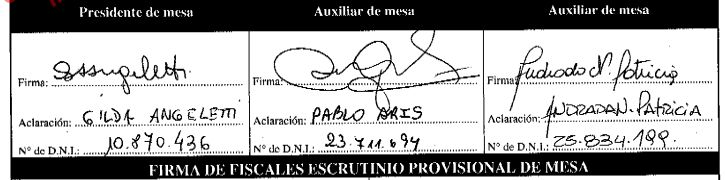
\includegraphics[width=0.75\textwidth]{imgs/telegramas2.png}
\end{center}
\end{subfigure}

\begin{subfigure}{0.45\textwidth}
\begin{center}
    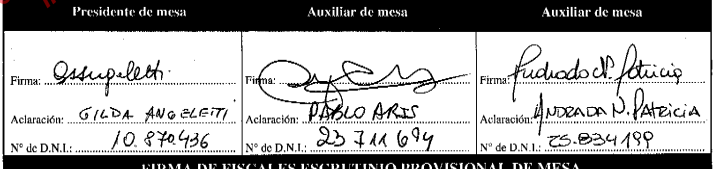
\includegraphics[width=0.75\textwidth]{imgs/telegramas3.png}
\end{center}
\end{subfigure}

\caption{ Recorte de la sección de firmas de dos páginas de un mismo telegrama. Para ver un telegrama completo ir al a figura \ref{fig:telegramas}. En las secciones donde aparecen firmas también aparecen otros trazos del formulario como la línea de puntos. Fuente: }
\label{fig:telegramas-firmas}
\end{figure}

\begin{figure}[h!]

\begin{subfigure}{0.45\textwidth}
\begin{center}
 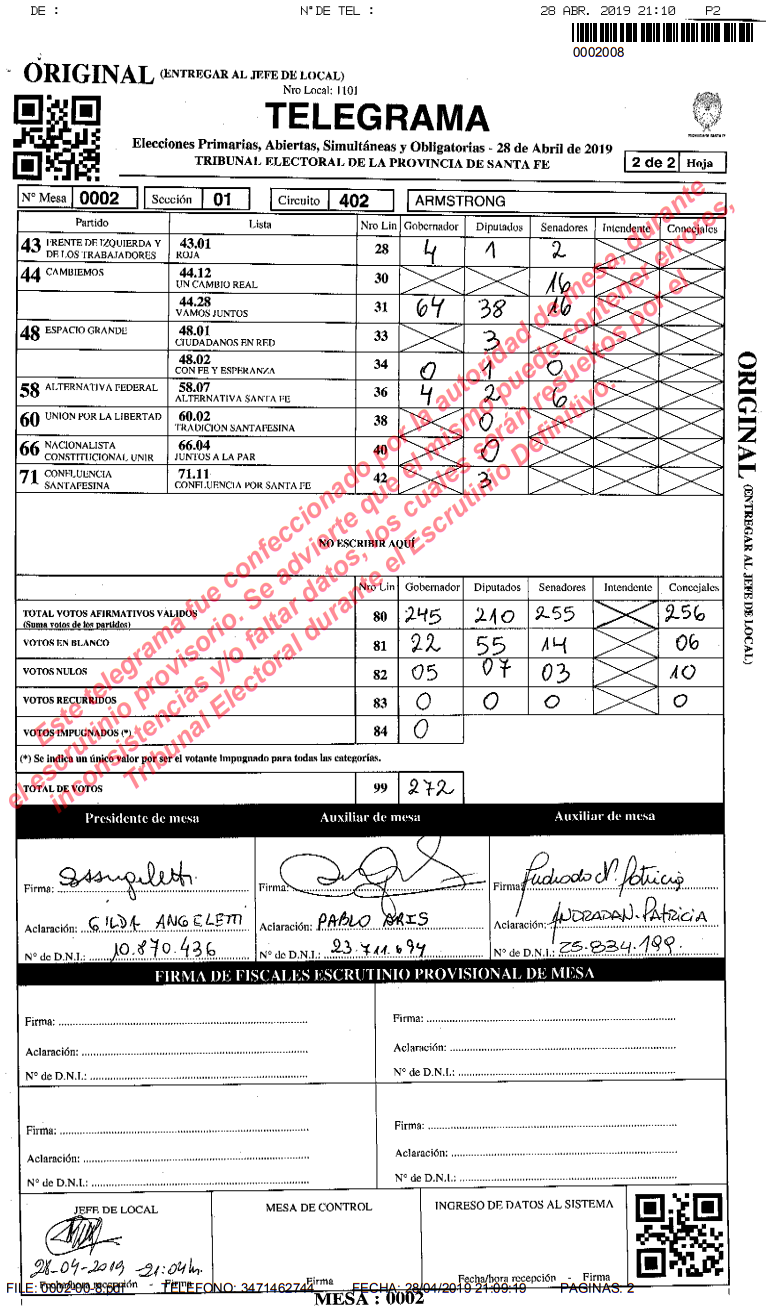
\includegraphics[width=0.85\textwidth]{imgs/telegramas1.png}
 \end{center}
\end{subfigure}

\caption{ Ejemplo de un telegrama electoral de las elecciones primarias de 2019. El formato es conocido meses antes de las elecciones. Los códigos QR de las esquinas sirven para enderezar las fotografías de los telegramas. Fuente: \cite{unr1} }
\label{fig:telegramas}
\end{figure}


Luego los telegramas son transmitidos al centro de cómputo del escrutinio provisorio. Operadores humanos llevan la labor de carga de datos, realizándose chequeos de consistencia. Si se detectan errores en esta fase puede pedírsele a las autoridades de la mesa que realicen nuevamente la confección del telegrama y/o  el recuento según sea necesario. Nos referiremos a estos eventos como \textbf{retransmisiones}. Las autoridades de mesa deben esperar la confirmación del centro de cómputo de que el telegrama ha sido chequeado y cargado para considerar su labor finalizada.


Según surge de las estadísticas del informe \cite{unr-informe} (sección 7.3), de poderse automatizar los procesos de:
\begin{enumerate}
    \item Detectar que firmas de las autoridades de mesa estén presentes y coincidan en todas las páginas de un mismo telegrama.
    \item Detectar los números en grillas de telegramas de votación (y hacer chequeos de consistencia, como por ejemplo verificación de totales).
\end{enumerate}
Se podrían introducir chequeos automáticos antes de que el telegrama sea enviado al centro de cómputo logrando:
\begin{itemize}
    \item  Aumentar la celeridad en la carga de telegramas en el centro de cómputo.
    \item Disminuir las solicitudes de reenvío de telegramas.
\end{itemize}
En definitiva, disminuir en gran medida el trabajo humano.\\

Nos enfoquermoes en el primer problema: reconocer firmas y constatar coincidencia entre ellas.

\section{Definiendo los objetivos}
\label{section:objectives}

Como veremos en el capítulo \ref{chapter:trabajos-anteriores}, existen variedad de problemas similares relativos a firmas manuscritas.

Como el diseño de los telegramas se conoce de antemano, y las firmas que se quieren analizar aparecen en posiciones determinadas de la página, no es necesario resolver el problema general de \textit{Signature Recognition}. Nos bastará recortar dicha sección de la página y determinar si hay o no una firma. Esto, hasta hace muy poco tiempo atrás consistía en un problema para nada trivial, sobretodo puesto que en la sección aparecen otros trazos como partes del formulario. No obstante, con el estado actual de los analizadores de imágenes hemos podido resolverlo sin demasiado ajetreo y hemos extendido y focalizado el trabajo de la tesina en el problema -mucho más desafiante- de similitud de firmas.\\

El problema de determinar si dos firmas son el mismo \textit{tipo de firmas} (fueron realizadas por el mismo autor) puede expresarse más formalmente como el predicado\footnote{En nuestro caso contamos con imágenes de las firmas manuscritas, pero existen otros ámbitos donde se cuenta también con información dinámica (temporal) acerca de cómo fue generado el trazo. También existen conjuntos de datos para este otro problema.}:
\begin{equation*}
    autoresCoinciden( firmaA : Imagen, firmaB : Imagen) \rightarrow Bool
\end{equation*}
Es así que el problema puede ser tratado como un problema de clasificación binaria donde las imágenes de ambas firmas constituyen la entrada.\\

Además, como se detalló en el apartado \ref{subsubsection:metricbinary}, al querer detectar \textit{no coincidencias} (ya que las mismas constituyen un error en la confección del telegrama analizado), trateremos a las mismas como clase positiva. Así nuestro clasificador tratará de computar la siguiente función:

\begin{equation*}
    autoresNoCoinciden( firmaA : Imagen, firmaB : Imagen) \rightarrow Bool
\end{equation*}

\subsection{Modelado del problema}

A diferencia del problema de \textit{signature verification} donde hay que determinar si una firma pertenece al autor que declara ser (conociendo previamente ciertas firmas para cada autor), en nuestro problema es posible (y probable) que las firmas sobre las que aplicaremos nuestra solución sean de autores completamente distintos a los que usamos para entrenar. Es por ello que no podemos entrenar un clasificador binario para cada autor como se hace en algunos trabajos relacionados.

Nuestra entrada serán pares de firmas y nuestra salida un booleano que indicará si es clasificado como coincidencia o no. Formalmente, una solución al problema consiste en un par de funciones:
\begin{itemize}
    \item $fit(firmas, clases)$: entrena la solución utilizando un conjunto de imágenes para las cuales se conocen sus respectivos autores.
    \item $predict(img_1, img_2) \rightarrow Bool$: determina si dos firmas son una coincidencia o no.
\end{itemize}

\subsection{Definición de los experimentos}
\label{subsection:definicion-experimentos}

Cada experimento consiste en una 3-upla $(dev, test, test\_ds)$:
\begin{itemize}
    \item \textbf{dev} y \textbf{test}: son duplas $(firmas, clases)$ con paths hacia imágenes y sus clases (autores) respectivamente. Los elementos de $dev$ se utilizan para entrenar.
    \item \textbf{test\_ds}: consiste en 3-uplas $(idx_1, idx_2, bool)$ donde el booleano determina si $test[idx_1]$ y $test[idx_2]$ constituyen un matcheo o no. Es importante usar las mismas 3-uplas para evaluar cada solución de modo que la comparación sea correcta.
\end{itemize}

\subsubsection{Desarrollo: entrenamiento y validación}

Del conjunto de firmas dedicadas al desarrollo ($dev$) se obtienen tanto los subconjuntos de entrenamiento (para encontrar los parámetros del modelo) como de validación (para encontrar los hiperparámetros).

La cantidad de clases (autores) distintas en el conjunto de desarrollo puede ser escasa. En dichos casos las métricas en validación pueden variar demasiado dependiendo de la elección de partición entrenamiento/validación, lo cual hace sensible a la elección de hiperparámetros. Es por eso que utilizamos un \textbf{5-fold cross validation} sobre el conjunto de desarrollo para generar 5 particiones, de modo que la elección de hiperparámetros sea más robusta.

Es importante, si vamos a comparar el score de validación de varios modelos, fijar también los emparejamientos de elementos (recordemos que nuestra solución toma pares) para los subconjuntos de validación.

\subsubsection{Construcción del conjunto de pares}

Al armar las parejas en los conjuntos de test y validación se construyen siempre conjuntos balanceados: hay tantas coincidencias como no coincidencias. Si se generaran todas las parejas posibles el conjunto contendría muchas más no coincidencias que coincidencias.

Para generar coincidencias, para cada clase se arman parejas sin repetirlas (sin considerar orden). Un parámetro $cls\_sampling\_limit$ limita la cantidad de veces que un elemento aparece en las parejas auténticas. Para generar pares no coincidentes se toma para cada elemento otros elementos no coincidentes (tantos como coincidentes) dejando el conjunto balanceado.

\subsection{Elección de la métrica}

El objetivo de los modelos es realizar una predicción lo más acertada posible. En la práctica, las predicciones se usan para tomar decisiones. Es así que los diferentes tipos de error no son equiparables. Como se vio en \ref{subsubsection:metricbinary} en el caso de la clasificación binaria tenemos \textit{falsos negativos} y \textit{falsos positivos}. \\

En nuestro caso, al aceptar pares de firmas que no coinciden (falsos negativos), el automatismo no cumplirá su objetivo de disminuir las retransmisiones y el trabajo humano innecesario. En caso de falsos positivos, las alarmas emitidas por el asistente serán incorrectas corriendo el riesgo de que el usuario desestime su opinión y que lejos de aumentar la eficiencia del proceso entorpezca la labor. \\

Es por esto que es importante no basarse en la tasa de aciertos (\textit{accuracy}), sino medir ambos errores de forma separada. Esto también es necesario cuando se trabaja con conjuntos de datos desbalanceados.\\

Para nuestro trabajo tomaremos como métrica a maximizar: ``la mayor \textit{precision} para la cuál el \textit{recall} sea mayor que 0.9''. Así, nuestra métrica tendrá un significado práctico: queremos que nuestro sistema capture el 90\% de los errores de firmas no coincidentes (reduciendo al 10\% el número de retransmisiones por esta causa) y que sea lo más fiable posible (en el sentido de que no genere falsas alarmas).

Habiendo calculado esta métrica, podría ser útil dar a conocer al usuario el umbral de \textit{precision}. Esto de alguna manera le indicará el ``grado de garantía'' que poseen las alarmas. Por ejemplo: si la \textit{precision} obtenida es del 0.8, nos dice que tan sólo alrededor de 1 de cada 5 alarmas son falsas.

\section{Conjuntos de datos utilizados}

\subsection{Experimento 1}

Para este experimento se utilizaron los datasets NISDCC y NFI (usados en SigComp 2009). NFI consta de 80 autores y NISDCC de 12 autores. Presumiblemente las diferencias entre ambos datasets son mayores que las diferencias internas de cada uno (en cuanto al tipo de trazo, calidad de las firmas, metodología de construcción).

Para el conjunto de test se deseó tener un número razonable de autores (al menos 30) y a la vez utilizar uno de los datasets exclusivamente para test:
\begin{itemize}
    \item 60 autores de NFI como conjunto de desarrollo.
    \item NISDCC + los 20 autores restantes de NFI como conjunto de test.
\end{itemize}

\subsection{Experimento 2}

Para este experimento se agregó a los datasets NISDCC y NFI el dataset de firmas CEDAR, aumentando significativamente el número de autores y firmas disponibles para desarrollo y evaluación.




